% ===============================================
% MATH 373: Intro to Numerical Analysis           Spring 2021
% prog_0_report.tex
% December 17, 2021
% ===============================================

% -------------------------------------------------------------------------
% You can ignore this preamble. Go on
% down to the section that says "START HERE" 
% -------------------------------------------------------------------------

\documentclass{article}

% load packages
\usepackage{amsmath,amsfonts,graphicx,amsthm,amssymb,hyperref,xcolor}

% Define default environments
\newenvironment{theorem}[2][Theorem]{\begin{trivlist}
\item[\hskip \labelsep {\bfseries #1}\hskip \labelsep {\bfseries #2.}]}{\end{trivlist}}
\newenvironment{lemma}[2][Lemma]{\begin{trivlist}
\item[\hskip \labelsep {\bfseries #1}\hskip \labelsep {\bfseries #2.}]}{\end{trivlist}}
\newenvironment{claim}[2][Claim]{\begin{trivlist}
\item[\hskip \labelsep {\bfseries #1}\hskip \labelsep {\bfseries #2.}]}{\end{trivlist}}
\newenvironment{problem}[2][Problem]{\begin{trivlist}
\item[\hskip \labelsep {\bfseries #1}\hskip \labelsep {\bfseries #2.}]}{\end{trivlist}}
\newenvironment{proposition}[2][Proposition]{\begin{trivlist}
\item[\hskip \labelsep {\bfseries #1}\hskip \labelsep {\bfseries #2.}]}{\end{trivlist}}
\newenvironment{corollary}[2][Corollary]{\begin{trivlist}
\item[\hskip \labelsep {\bfseries #1}\hskip \labelsep {\bfseries #2.}]}{\end{trivlist}}

\newenvironment{solution}{\begin{proof}[Solution]}{\end{proof}}

%adjust to 1 in margins
  \addtolength{\oddsidemargin}{-.875in}
   \addtolength{\evensidemargin}{-.875in}
    \addtolength{\textwidth}{1.75in}

    \addtolength{\topmargin}{-.875in}
    \addtolength{\textheight}{1.75in}
    
    
% Define Shortcuts
\def\ds{\displaystyle}
\def\beginrefs{\begin{list}%
        {[\arabic{equation}]}{\usecounter{equation}
         \setlength{\leftmargin}{2.0truecm}\setlength{\labelsep}{0.4truecm}%
         \setlength{\labelwidth}{1.6truecm}}}
\def\endrefs{\end{list}}
\def\bibentry#1{\item[\hbox{[#1]}]}

\begin{document}



% ------------------------------------------ %
%                 START HERE             %
% ------------------------------------------ %

\large

{\Large Math 373, Introduction to Numerical Analysis}

\begin{center}
{\Large Author: \hfill Kyle Riley} 
\end{center}
\par \medskip \par
{\Large Programming Assignment: 0}  
\par \bigskip \par

% Complete summary and remove the instructions in red
{\bf Summary:} This program is designed to calculate the Taylor's Polynomial for $\ln(x)$ with the user supplying the center, the point to be approximated, and the degree of the polynomial. The program is to return a flag, the approximated value, and the absolute relative error. The flag=0 implies the program ran without error, flag = 1 implies the program concluded with an error, and flag = 2 implies the method diverged. If an approximation cannot be calculated the program should return -666 and if the relative error cannot be calculated then the program should return rel = -1.  The program that has been submitted for evaluation is progz12456.m and it should be in the m-file dropbox for this assignment. 
\par \bigskip \par

% Complete methods and remove the instructions in red
{\bf Methods:} The central calculation for this method is the Taylor's Polynomial for $\ln(x)$, which was found to be
$$P_n(x) = \ln(x_0) + \sum_{k=1}^n\frac {(-1)^{k+1}}{k*x_0^k}(x-x_0)^k,$$
the $\ds (-1)^{k+1}$ term is used to produce the alternating sign value with odd terms being positive and even terms to be negative. The assignment did not specifically indicate that the input for $x$ or for $x_0$ would be positive and so a check was installed to make sure both $x$ and $x_0$ were positive. The assignment also did not specify that n was an integer and so the program incorporated the natural use of MATLAB that if n was a fractional value then the closest integer smaller than $n$ was used for the expansion. If the user desired use of $n$ that were not integer then more detailed information on the related calculation would be needed. The assignment clearly specified that input would be numerical and that $n$ would be positive , which translates into no further screening on the input values from the user. 

The relative error calculation is not possible if the exact value is equal to zero and so an if statement was used to screen for cases where the exact value is zero. This procedure should be altered if there is a desire to secure calculations where the exact is very near zero, but not equal to zero. The Taylor approximation can diverge and so a simple if statement is used to screen cases where the approximation diverges in MATLAB to NaN, which is a way to identify divergence. An alternative to using NaN is to cap abs(approx) by a sufficiently large value that would be associated with divergence. 
\par \bigskip \par


% Complete testing and analysis, please remove the instructions in red
{\bf Testing and Analysis:} Small simple cases that can be replicated by hand were used to validate the calculations were correct (these cases are given in the appendix). Input of nonpositive values for $x$ and $\ds x_0$ were used to test the screen for faulty input and the use of non-integer values for $n$ where also used to test the program under these conditions. The testing did include a test of the screen for relative error to prevent division by the exact value being equal to zero. Lastly, a case of divergence was found to test the program screen for divergence. 
\par \bigskip \par

%Hit list is optional, but is evidence of higher learning, developing strong skills in reviewing are extremely valuable. Please remove instructions in red.
{\bf Hit List: }This program addresses the specific requirements of the assignment. As noted earlier, non-integer values of $n$ are allowed in this program and the approaches for handling relative error and divergence are implemented in very exacting strategies. Both relative error and divergence could be developed with more robust approaches if needed. The program does screen for nonpositive values for $x$ and $\ds x_0$, but numerically it might be useful to identify the positive thresholds that would be needed to limit $x$ and $\ds x_0$. 
\par \bigskip \par


{\bf Academic Integrity}: {\color{red} The goal of this assignment is that everyone write their own code. This means you should not copy any code from any other source (the only exception are the templates provided by the instructor.) If you copy any code then you are in violation of integrity specifications of this assignment. If you provide your code to others then you are also in violation of the integrity rules of this assignment.  }


I affirm that this program submission complies with the integrity specifications of this assignment. I understand if I am in violation of the integrity specification then I will get a zero on the assignment and receive an overall reduction in my course grade by one letter grade. 

% Add references here, list alphabetically according to last name of primary author.
\section*{References}
\beginrefs


\bibentry{LB16}{\sc Leon Brin},
{\it Tea Time Numerical Analysis (Experiences in Mathematics)  (2nd ed.)}, 2016. Website: \href{http://lqbrin.github.io/tea-time-numerical/}{lqbrin.github.io/tea-time-numerical} .

\bibentry{Matlab} {\sc Matlab website}, \href{https://www.mathworks.com}{www.mathworks.com}, August 2019. % put exact and full link in the first listing right after href

\bibentry{KR20} {\sc Kyle Riley}, Class Lecture, Math 373: Introduction to Numerical Analysis, Lecture, January 2020. 

\endrefs

\bigskip \par \bigskip
%%%------------------------------------------------------
%  Appendix, remove the red comments when completing this section. 
%%----------------------------------------------------------
{\Large {\bf Appendix}} \par \medskip
There was significant work in testing, but to capture a few of the main points would include the following.

The work to validate the calculations are correct was done using small numbers that can be duplicated by hand using a calculator or a spreadsheet. For example, the case of $\ds x_0= 1$, $x=1.2$, and $n=3$ results in:
\begin{verbatim}
>> [flag, approx, rel]= progz123456(1,1.2,3);
>> [flag, approx, rel]
         0    0.1827    0.0019
\end{verbatim}
which is confirmed by calculations by hand to have the same value. Another example, $x_0=2$, $x=1.7$, and $n=4$ results in:
\begin{verbatim}
>> [flag, approx, rel]= progz123456(2,1.7,4);
>> [flag, approx, rel]
         0    0.5306    0.0000
\end{verbatim}
which was also confirmed by a spreadsheet calculation. Another validation is the replication of convergence, which can be seen with $\ds x_0=1$, $x=1.8$ and increasing values of $n$
\begin{verbatim}
>> [flag, approx, rel]= progz123456(1,1.8,5);
>> [flag, approx, rel]
         0    0.6138    0.0443
         
>> [flag, approx, rel]= progz123456(1,1.8,15);
>> [flag, approx, rel]
         0    0.5888    0.0017

>> [flag, approx, rel]= progz123456(1,1.8,25);
>> [flag, approx, rel]
         0    0.5879    0.0001
\end{verbatim}
this shows that the method does converge for a case where it should converge. 

A test of divergence can be given by: $\ds x_0 = 1$, $x=10.5$, and $n=500$
\begin{verbatim}
>> [flag, approx, rel]= progz123456(1,10.5,500);
>> [flag, approx, rel]
     2  -666    -1
\end{verbatim}

Tests for screening bad input include: 
$\ds x_0=0$
\begin{verbatim}
>> [flag, approx, rel]= progz123456(0,1.7,4);
>> [flag, approx, rel]
     1  -666    -1
\end{verbatim}
$x=-1.1$
\begin{verbatim}
>> [flag, approx, rel]= progz123456(1,-1.1,4);
>> [flag, approx, rel]
     1  -666    -1
\end{verbatim}
As noted earlier, non-integer positive values for $n$ are allowed and so a test of this can be found in: with $\ds x_0=1$, $x=1.4$, and $n=4.7$
\begin{verbatim}
>> [flag, approx, rel]= progz123456(1,1.4,4.7);
>> [flag, approx, rel]
         0    0.3349    0.0046
\end{verbatim}
which really reduces to an expansion for $n=4$. 

The last test to mention is the screen for relative error, which breaks down in the case when the exact value is equal to zero. A simple test for this screen is the case: $\ds x_0 = 1.3$, $x=1$, and $n=10$. The result is given by:
\begin{verbatim}
>> [flag, approx, rel]= progz123456(1.3,1,10);
>> [flag, approx, rel]
    1.0000    0.0000   -1.0000
\end{verbatim}

\vfill \eject
{\color{teal}
{\bf Note on using Figures in LaTeX}}

LaTeX is really a wonderful tool that has tremendous power to create beautiful technical documents, but one area that produces consistent frustration is how LaTeX handles figures. In the end, it is not possible to exercise complete control regarding the placement of figures. There are several tricks and strategies that one can develop, but LaTeX is rather independent on placement of figures. A few examples are given below to illustrate how to import figures into a document. 

It is possible to bring in an image without making it a formal figure in the document. This can be accomplished in a variety of ways, but the one we will illustrate is a direct reference via the include graphics command. The command $\backslash$includegraphics[width=100m]{graphics\_1.png} loads the figure from the file graph\_1.png and sets the width of the figure as 100 mm, which results in:  


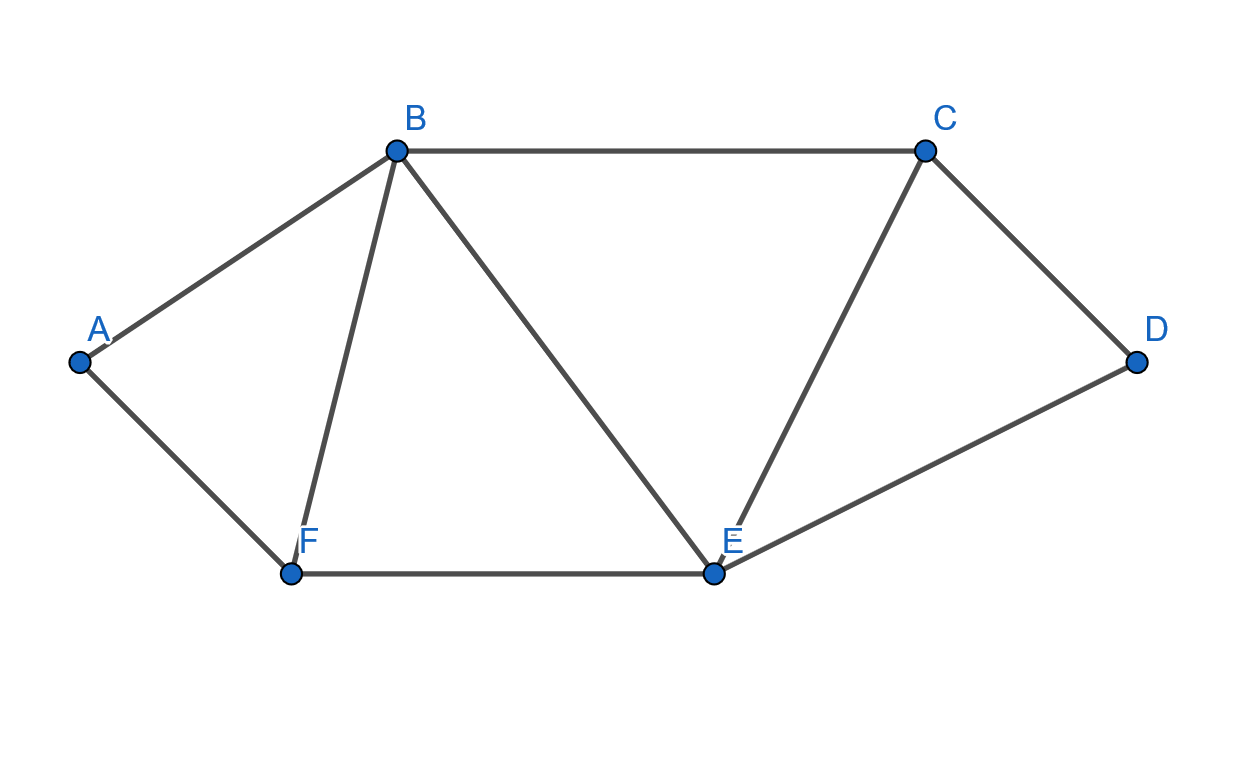
\includegraphics[width=100mm]{graph_1.png}

Classic LaTeX could only incorporate images that were files formatted as encapsulated postscript (*.eps) files. Matlab can still generate encapsulated postscript files, but LaTeX has evolved into being able to include several different file types, although different file types might require different LaTeX commands to produce desired results. The true way to import an image into a document is to include it as a figure. This requires the figure environment and it is started with begin$\{$figure$\}$ and is concluded with end$\{$figure$\}$. An illustration of the figure command is:
\begin{verbatim}
\begin{figure}[!ht]
\centering  %centering can be used to center the image

\includegraphics[height=50mm]{grubby.jpg}
 \caption{Image of Grubby}
 \label{f:grubby}
\end{figure}
\end{verbatim}
The result is the image along with a caption, plus the label enables the author to refer to this Figure later in the document. 
\medskip

\begin{figure}[!ht]
\centering  %centering can be used to center the image

\includegraphics[height=50mm]{grubby.jpg}
 \caption{Image of Grubby}
 \label{f:grubby}
\end{figure}

The great thing about using the figure environment is that it includes several options. An author can add a caption to a figure and it is best practice to add a caption to any figure you place in a document. In addition, you can add an internal label to a figure and then be able to reference the figure by that label. For example, 'Figure $\backslash$ref$\{$f:grubby$\}$' results in: Figure \ref{f:grubby}, and this can reference the same figure and the numbers will automatically be updated no matter how many figures are added into the document. This makes it very flexible for the author to manage figures in a document and if LaTeX decides to place a figure on a different page then the author can always refer to a specific image by the label, which is another best practice to keep in mind. 

Generally, images will align to the left of the page. It is possible to move images to align left, center, or to the right and there are a variety of packages and commands to make such a move happen. It is important to know what is exactly in the image file since some files include a great deal of white space around the given image. It might become necessary for you to crop an image before you include it in a document. An example of changing alignment can be illustrated by:
\begin{verbatim}
\begin{figure}[!ht]
\begin{flushright}
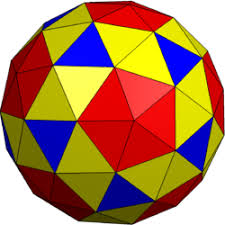
\includegraphics[height=50mm]{dodecahedron.jpg}
 \caption{Dodecahedron (image aligned right)}
 \label{f:dodecahedron}
 \end{flushright}
\end{figure} 
\end{verbatim}

\begin{figure}[!ht]
\begin{flushright}
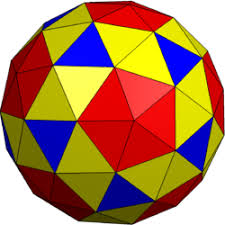
\includegraphics[height=50mm]{dodecahedron.jpg}
 \caption{Dodecahedron (image aligned right)}
 \label{f:dodecahedron}
 \end{flushright}
\end{figure}

Figure \ref{f:dodecahedron} produces the figure with alignment right. 

\medskip 

Lastly, it is possible to draw figures directly in LaTeX. This process is tedious and much like programming an etch a sketch, but the nice part is that everything is contained and controlled in LaTeX and would not require any external files. LaTeX has many features and commands that work with figures, but the requirements in Math 373 will require very basic use of images and figures.

% ---------------------------------------------------
% Anything after the \end{document} will be ignored by the typesetting.
% ----------------------------------------------------

\end{document}